%\documentclass[aps,prb,twocolumn,superscriptaddress,footinbib,amsmath,amssymb,floatfix]{revtex4}
\documentclass[aps,prb,onecolumn,preprint,superscriptaddress,footinbib,amsmath,amssymb,floatfix]{revtex4}
\usepackage[dvips]{epsfig}
\usepackage{graphicx}
\usepackage{ifthen}
\usepackage{dcolumn}% Align table columns on decimal point
\usepackage{bm}% bold math
\usepackage{multirow}
\usepackage{booktabs}
\usepackage{bm}% bold math
\usepackage{amsbsy}
\usepackage{amsmath}
\usepackage{amssymb}
\usepackage{subfigure}
%\usepackage{wrapfig}

%Definition of new commands
\newcommand{\f}[2]{\ensuremath{\frac{\displaystyle{#1}}{\displaystyle{#2}}}}
\newcommand{\lr}[1]{\langle{#1}\rangle}
\newcommand{\colv}[2] {\left(\begin{array}{c} #1 \\ #2 \end{array}\right)}
\renewcommand{\thefootnote}{\fnsymbol{footnote}}
\newcommand{\be} {\begin{eqnarray}}
\newcommand{\ee} {\end{eqnarray}}
%--------------------------------------------------------------------------
%EQ COMMANDS
%--------------------------------------------------------------------------
\newcommand{\two}{\mspace{-2.0mu}}
\newcommand{\four}{\mspace{-4.0mu}}
\newcommand{\plus}{\mspace{-4.5mu}+\mspace{-3.5mu}}
\newcommand{\minus}{\mspace{-4.5mu}-\mspace{-3.5mu}}
\newcommand{\pp}{'\mspace{-2.0mu}'}
\newcommand{\xlb}[4]{#1\ifthenelse{\equal{#2}{0}}{}{_{\alpha #2}}
\mspace{-2.0mu}\genfrac{(}{)}{0pt}{1}{\ifthenelse{\equal{#3}{0}}{0}{l #3}} 
{\ifthenelse{\equal{#4}{0}}{0}{b #4}}}

\newcommand{\xkv}[4]{#1\mspace{-5.0mu}\left(\mspace{-8.0mu}
\begin{smallmatrix}#2\four{}\four{}\mspace{-8.0mu}&\pmb{\kappa}#3\\&\nu 
#4\end{smallmatrix}\mspace{-5.0mu}\right)}

\newcommand{\evect}[6]{#1\mspace{-4.0mu}\left(\mspace{-8.0mu}
\begin{smallmatrix}#2\mspace{-8.0mu}&\pmb{\kappa} #3 &b #5\\&\nu #4 &
\alpha #6\end{smallmatrix}\mspace{-5.0mu}\right)}

\newcommand{\varmat}[8]{\mspace{-5.0mu}\left(\mspace{-8.0mu}
\begin{smallmatrix}\ifthenelse{\equal{#3}{0}}{\mspace{-8.0mu}&b_{#1}&b_{#2}
\\&\alpha_{#1}&\alpha_{#2}} {\ifthenelse{\equal{#7}{0}}{#1\mspace{-8.0mu}&
\pmb{\kappa}#2#3\mspace{-8.0mu}&\pmb{\kappa}#4#5\mspace{-8.0mu}&\pmb{\kappa}
#6\\&\nu#2&\nu#4&\nu#6} {#1\mspace{-8.0mu}&\pmb{\kappa}#2#3\mspace{-8.0mu}&
\pmb{\kappa}#4#5\mspace{-8.0mu}&\pmb{\kappa}#6#7\mspace{-8.0mu}&\pmb{\kappa}
#8\\&\nu#2&\nu#4&\nu#6&\nu#8}}\end{smallmatrix}\mspace{-5.0mu}\right)}

\newcommand{\EXP}[1]{\exp\mspace{-5.0mu}\left[#1\right]\mspace{-3.0mu}}

\newcommand{\tpp}[2]{\left(\mspace{-2.0mu}\xkv{\omega}{}{}{}#1\xkv{\omega}
{}{'}{'}#2\xkv{\omega}{}{\pp}{\pp}\mspace{-2.0mu}\right)}



%--------------------------------------------------------------------------
\newcommand{\SUM}[2]{\ifthenelse{\equal{#1}{0}}{\sum_{
\alpha_{#2},b_{#2},l_{#2}}^{3,n,N}} {\ifthenelse{\equal{#1}{1}}{\sum_{
\alpha_{#2},b_{#2}}^{3,n}}{\sum_{\pmb{\kappa}#2,\nu#2}^{N,3n}}}}

\newcommand{\SUMprime}[2]{\ifthenelse{\equal{#1}{0}}
{\sum_{\alpha_{#2},b_{#2},l_{#2}}^{3,n,N}} 
{\ifthenelse{\equal{#1}{1}}{\sum_{\alpha_{#2},b_{#2}}^{3,n}}
{\sum_{\pmb{\kappa}^{'}#2,\nu#2}^{N,3n}}}}

\newcommand{\SUMalpha}[2]{\ifthenelse{\equal{#1}{0}}
{\sum_{\alpha_{#2}}^{3}} {\ifthenelse{\equal{#1}{1}}
{\sum_{\alpha_{#2},b_{#2}}^{3,n}}{\sum_{\pmb{\kappa}#2,\nu#2}^{N,3n}}}}
%--------------------------------------------------------------------------
\newcommand{\SUMalphap}[2]{\ifthenelse{\equal{#1}{0}}
{\sum_{\alpha'_{#2}}^{3}} {\ifthenelse{\equal{#1}{1}}
{\sum_{\alpha'_{#2},b'_{#2}}^{3,n}}{\sum_{\pmb{\kappa}#2,\nu#2}^{N,3n}}}}

\newcommand{\SUMb}[2]{\ifthenelse{\equal{#1}{0}}{\sum_{b_{#2}}^{n}}
 {\ifthenelse{\equal{#1}{1}}{\sum_{\alpha_{#2},b_{#2}}^{3,n}}
{\sum_{\pmb{\kappa}#2,\nu#2}^{N,3n}}}}

\newcommand{\SUMbp}[2]{\ifthenelse{\equal{#1}{0}}{\sum_{b'_{#2}}^{n}}
 {\ifthenelse{\equal{#1}{1}}{\sum_{\alpha'_{#2},b'_{#2}}^{3,n}}
{\sum_{\pmb{\kappa}#2,\nu#2}^{N,3n}}}}

\newcommand{\SUMl}[2]{\ifthenelse{\equal{#1}{0}}{\sum_{l_{#2}}^{N}}
 {\ifthenelse{\equal{#1}{1}}{\sum_{\alpha_{#2},b_{#2}}^{3,n}}
{\sum_{\pmb{\kappa}#2,\nu#2}^{N,3n}}}}

\newcommand{\SUMlp}[2]{\ifthenelse{\equal{#1}{0}}{\sum_{l'_{#2}}^{N}}
 {\ifthenelse{\equal{#1}{1}}{\sum_{\alpha'_{#2},b'_{#2}}^{3,n}}
{\sum_{\pmb{\kappa}#2,\nu#2}^{N,3n}}}}

\newcommand{\abcdt}[5]{\mspace{-4.0mu}\left(\mspace{-8.0mu}
\begin{smallmatrix}&\ifthenelse{\equal{#1}{}}{a}{#1}&\ifthenelse
{\equal{#3}{}}{c}{#3}\\&\ifthenelse{\equal{#2}{}}{b}{#2}&\ifthenelse
{\equal{#4}{}}{d}{#4}\end{smallmatrix}\mspace{-2.0mu};\ifthenelse
{\equal{#5}{}}{t}{#5}\right)}

\newcommand{\abcd}[4]{\mspace{-4.0mu}\left(\mspace{-8.0mu}
\begin{smallmatrix}&\ifthenelse{\equal{#1}{}}{a}{#1}&\ifthenelse
{\equal{#3}{}}{c}{#3}\\&\ifthenelse{\equal{#2}{}}{b}{#2}&\ifthenelse
{\equal{#4}{}}{d}{#4}\end{smallmatrix}\mspace{-3.0mu}\right)}

\newcommand{\abt}[3]{\mspace{-4.0mu}\left(\mspace{-8.0mu}\begin
{smallmatrix}&\ifthenelse{\equal{#1}{}}{a}{#1} \\&\ifthenelse{
\equal{#2}{}}{b}{#2}\end{smallmatrix}\mspace{-2.0mu};
\ifthenelse{\equal{#3}{}}{t}{#3}\right)}

\newcommand{\ab}[2]{\mspace{-4.0mu}\left(\mspace{-8.0mu}
\begin{smallmatrix}&\ifthenelse{\equal{#1}{}}{a}{#1} \\&\ifthenelse
{\equal{#2}{}}{b}{#2}\end{smallmatrix}\mspace{-3.0mu}\right)}

\newcommand{\kvbat}{\mspace{-4.0mu}\left(\mspace{-8.0mu}
\begin{smallmatrix} &\pmb{\kappa} &b \\ &\nu &\alpha\end{smallmatrix}
\mspace{-2.0mu};t\right)}
%--------------------------------------------------------------------------


\newcommand{\kgvba}{\mspace{-4.0mu}\left(\mspace{-8.0mu}
\begin{smallmatrix} &\pmb{\kappa}=\pmb{0} &b \\ &\nu 
&\alpha\end{smallmatrix}\mspace{-3.0mu}\right)}

\newcommand{\kgv}{\mspace{-4.0mu}\left(\mspace{-8.0mu}
\begin{smallmatrix}&\pmb{\kappa}=\mathbf{0} \\&\nu\end{smallmatrix}
\mspace{-3.0mu}\right)}

%--------------------------------------------------------------------------

\newcommand{\kvbatp}{\mspace{-4.0mu}\left(\mspace{-8.0mu}
\begin{smallmatrix} &\pmb{\kappa} &b' \\ &\nu &\alpha'\end{smallmatrix}
\mspace{-2.0mu};t\right)}

\newcommand{\kvbaw}{\mspace{-4.0mu}\left(\mspace{-8.0mu}
\begin{smallmatrix} &\pmb{\kappa} &b \\ &\nu &\alpha\end{smallmatrix}
\mspace{-2.0mu};\omega\right)}

\newcommand{\kvbawp}{\mspace{-4.0mu}\left(\mspace{-8.0mu}
\begin{smallmatrix} &\pmb{\kappa} &b' \\ &\nu &\alpha'\end{smallmatrix}
\mspace{-2.0mu};\omega\right)}

\newcommand{\kvba}{\mspace{-4.0mu}\left(\mspace{-8.0mu}
\begin{smallmatrix} &\pmb{\kappa} &b \\ &\nu &\alpha\end{smallmatrix}
\mspace{-3.0mu}\right)}

\newcommand{\kvbap}{\mspace{-4.0mu}\left(\mspace{-8.0mu}
\begin{smallmatrix} &\pmb{\kappa} &b' \\ &\nu &\alpha'\end{smallmatrix}
\mspace{-3.0mu}\right)}
%--------------------------------------------------------------------------
\newcommand{\kpvba}{\mspace{-4.0mu}\left(\mspace{-8.0mu}
\begin{smallmatrix} &\pmb{\kappa}^{'} &b \\ &\nu &\alpha\end{smallmatrix}
\mspace{-3.0mu}\right)}

\newcommand{\kva}{\mspace{-4.0mu}\left(\mspace{-8.0mu}
\begin{smallmatrix} &\pmb{\kappa} \\ &\nu &\alpha\end{smallmatrix}
\mspace{-3.0mu}\right)}

\newcommand{\kvap}{\mspace{-4.0mu}\left(\mspace{-8.0mu}
\begin{smallmatrix} &\pmb{\kappa} \\ &\nu &\alpha'\end{smallmatrix}
\mspace{-3.0mu}\right)}

\newcommand{\kvb}{\mspace{-4.0mu}\left(\mspace{-8.0mu}
\begin{smallmatrix} &\pmb{\kappa} &b \\ &\nu \end{smallmatrix}
\mspace{-3.0mu}\right)}

\newcommand{\kvbp}{\mspace{-4.0mu}\left(\mspace{-8.0mu}
\begin{smallmatrix} &\pmb{\kappa} &b' \\ &\nu \end{smallmatrix}
\mspace{-3.0mu}\right)}

\newcommand{\kvt}{\mspace{-4.0mu}\left(\mspace{-8.0mu}
\begin{smallmatrix}&\pmb{\kappa} \\&\nu\end{smallmatrix}
\mspace{-2.0mu};t\right)}

\newcommand{\kgvt}{\mspace{-4.0mu}\left(\mspace{-8.0mu}
\begin{smallmatrix}&\pmb{\kappa=0} \\&\nu\end{smallmatrix}
\mspace{-2.0mu};t\right)}

\newcommand{\kpvt}{\mspace{-4.0mu}\left(\mspace{-8.0mu}
\begin{smallmatrix}&\pmb{\kappa}^{'} \\&\nu\end{smallmatrix}
\mspace{-2.0mu};t\right)}

\newcommand{\kvw}{\mspace{-4.0mu}\left(\mspace{-8.0mu}
\begin{smallmatrix}&\pmb{\kappa} \\&\nu\end{smallmatrix}
\mspace{-2.0mu};\omega\right)}

\newcommand{\kv}{\mspace{-4.0mu}\left(\mspace{-8.0mu}
\begin{smallmatrix}&\pmb{\kappa} \\&\nu\end{smallmatrix}
\mspace{-3.0mu}\right)}

\newcommand{\kw}{\mspace{-4.0mu}\left(\mspace{-8.0mu}
\begin{smallmatrix}&\pmb{\kappa} \\&\omega\end{smallmatrix}
\mspace{-3.0mu}\right)}

\newcommand{\kpvp}{\mspace{-4.0mu}\left(\mspace{-8.0mu}
\begin{smallmatrix}&\pmb{\kappa'} \\&\nu'\end{smallmatrix}
\mspace{-3.0mu}\right)}
%--------------------------------------------------------------------------
\newcommand{\lbt}{\mspace{-4.0mu}\left(\mspace{-8.0mu}
\begin{smallmatrix}&l \\&b\end{smallmatrix}\mspace{-2.0mu};t\right)}

\newcommand{\lbtp}{\mspace{-4.0mu}\left(\mspace{-8.0mu}
\begin{smallmatrix}&l' \\&b'\end{smallmatrix}\mspace{-2.0mu};t\right)}

\newcommand{\lt}{\mspace{-4.0mu}\left(\mspace{-8.0mu}
\begin{smallmatrix}&l\end{smallmatrix}\mspace{-2.0mu};t\right)}

\newcommand{\ltp}{\mspace{-4.0mu}\left(\mspace{-8.0mu}
\begin{smallmatrix}&l'\end{smallmatrix}\mspace{-2.0mu};t\right)}

\newcommand{\lb}{\mspace{-4.0mu}\left(\mspace{-8.0mu}
\begin{smallmatrix}&l \\&b\end{smallmatrix}\mspace{-3.0mu}\right)}

\newcommand{\lbp}{\mspace{-4.0mu}\left(\mspace{-8.0mu}
\begin{smallmatrix}&l' \\&b'\end{smallmatrix}\mspace{-3.0mu}\right)}
%--------------------------------------------------------------------------
%COMMANDS
%--------------------------------------------------------------------------
\begin{document}
%--------------------------------------------------------------------------
\title{Origin of the Exceptionally-Low Thermal Conductivity of 
Fullerene-Derived PCBM Thin Films}
%--------------------------------------------------------------------------
\author{Jason M. Larkin}
\author{Alan J. H. McGaughey}
\affiliation{Department of Mechanical Engineering\\
Carnegie Mellon University\\Pittsburgh, PA 15213}
%\email[]{mcgaughey@cmu.edu}
%--------------------------------------------------------------------------
\date{\today}
%--------------------------------------------------------------------------
\begin{abstract}



\end{abstract}
%--------------------------------------------------------------------------
\maketitle
%--------------------------------------------------------------------------
\clearpage
\section{\label{S:Introduction}Introduction}
%--------------------------------------------------------------------------

Phase change random access memory (PRAM) is unique among semiconductor 
devices because heat is intrinsic to the operation of the device, not 
just a by-product. Here, we apply a material that is exotic in the 
context of typical semiconductor devices but has highly desirable 
properties for PRAM. Thin films of C60 are semiconducting and show very 
low thermal conductance. By inserting a C60 layer between the phase 
change material and the metal electrode, we dramatically reduced the heat 
dissipation and, thereby, the operating current. A PRAM device 
incorporating a C60 layer operated stably for more than 105 cycles.
\cite{kim_fullerene_2008}

A novel type of multi-layer vacuum insulation based on carbon 
nano-materials, namely fullerenes, has been demonstrated. The design 
is based on unique thermal insulation properties of fullerenes, arising 
from their electronic structure, as well as proprietary deposition 
technique using thin layers of reflective material as a support. As a 
result of experimental testing, the fabricated samples of fullerene-based 
insulation were shown to possess R-values of 36 to 40 per inch of 
thickness at cryogenic temperatures, which considerably exceeds those 
of commonly available insulation materials (for example, polyurethane 
(R6.7), expanded polystyrene (R3.8), and even vacuum insulated panels 
(R9∼24)). Application of such insulation will result in significant size 
and weight reduction while maintaining cost-effectiveness.
\cite{wexler_thermal_2004}

We have argued that our sample of C60 exhibits a substan-
tial amount of disorder. An indication of this is given by the
phonon mean free path. The mean free path l can be esti-
mated using the simple Debye formula for ␭ which is given
by ␭ϭ(1/3) ␳ c v l ␯ , where ␯ is the phonon velocity and ␳ c v is
the heat capacity per unit volume of the phonons which are
responsible for the heat transport. We associate the vibrating
unit with the C60 molecule ͑c v ϭ25 J molϪ1 KϪ1, ␳ϭ2400
mol mϪ3͒ and approximate ␯ with the sound velocity
͑Ϸ2ϫ103 m sϪ1͒, which yields lϭ50 Å at 200 K ͑about three
lattice constants͒. Although the absolute value for l obtained
in this way needs to be treated with caution, the true l is
almost certainly rather small. It probably follows that the
amount of defects must be substantial but a quantification is
not possible without specific knowledge of their ability to
scatter phonons.
\cite{andersson_thermal_1995}

Using a microcalorimeter, we have measured the specific heat of C60 
and K3 C60 thin films from 6–400 K.
The results can be understood by analyzing the phonon modes; the 
electronic specific heat of K3C60 is a small
fraction of the total. While C60 displays a clear separation of 
energy levels between interball and intraball
modes, the added ͑alkali͒ optical modes in K3C60 blur this separation 
because they appear in the gap. Addi-
tionally, the acoustic modes of K3 C60 soften compared to pure C60.
\cite{allen_specific_1999}

The phonon component
(0)
ϭ55.4 K)
is evaluated on the basis of the Debye model using the Debye temperature 
(⌰ D ̈ neisen parameters are
calculated from the known sound velocities. The general and partial Gru
calculated as functions of temperature. The results obtained for the 
high-temperature
phase indicate that rotations of C60 molecules are strongly hindered 
and intercorrelated.
\cite{aksenova_analysis_1999}

Using a novel microcalorimeter, we have performed the first specific heat 
measurements of C84 ,
Sc2 @C84 , C82 , and La@C82 ͑10–300 K͒. We analyze these results using a 
framework based on the
phonon modes in these materials. C84 compares qualitatively to C60 with a 
clear separation between
inter- and intraball modes, although the interball modes are significantly 
softer in C84 . For Sc2 @C84
the added optical modes due to the metal atoms are high-energy Einstein 
modes comparable to the
on-ball modes. Thus, the specific heat of Sc2 @C84 is very similar to that 
of C84 ; and likewise, the
specific heat of La@C82 resembles that of C82 . Remarkably, however, C82 
contrasts sharply with
the other empty fullerenes in that it shows no separation of energy levels 
between inter- and intraball
modes. We speculate about possible causes of this anomalous behavior.
In conclusion, we have shown from specific heat experi-
ments that C84 behaves qualitatively like C60 in terms of a
separation of energy levels between interball and intraball
modes. Thus, C84 is a molecular solid like C60 with weak
bonds between the balls and strong bonds on the balls. How-
ever, C84 shows significantly softer interball modes than C60 ,
saturating by 10 K, implying that the highest energy interball
modes are below 1 eV. Adding Sc inside the balls to make
Sc2 @C84 makes almost no difference to C p because the Sc
optical modes are high-energy modes that add into the intra-
ball modes instead of appearing in the gap as they do for
K3 C60 . 16 C82 , however, differs even more severely from the
other pure fullerenes studied. It shows no two-tiered behav-
ior in C p , and hence no separation of energy levels. La@C82
actually shows somewhat more separation of energy levels
than pure C82 due, we suggest, to a stiffening of low-energy
on-ball modes from the La–C bond, but it too has no true
separation of energy levels.
\cite{allen_specific_1999}

%--------------------------------------------------------------------------
\section{\label{S:Theory}Theoretical Formulation}
%--------------------------------------------------------------------------

%--------------------------------------------------------------------------
\subsection{\label{S:Theory:Thermal}Vibrational Thermal Conductivity}
%--------------------------------------------------------------------------

\begin{equation}\label{EQ:kvib}
\begin{split}
k_{vib} = k_{ph} + k_{AF},
\end{split}
\end{equation}


%--------------------------------------------------------------------------
\begin{figure}
\begin{center}
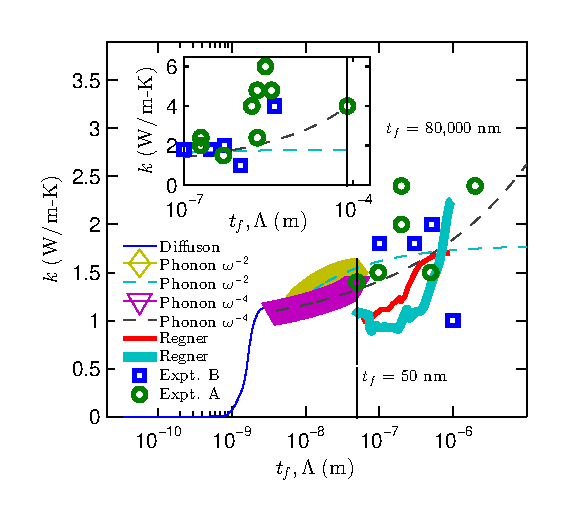
\includegraphics[scale=1.0]
{/home/jason/disorder/si/amor/m_af_si_normand_4096_kLamba_4_si.eps}
\vspace*{-5mm}
\end{center}
\caption{\label{FIG:accum} film thickness dependant thermal 
conductivity of a-Si from experiment.}
\end{figure}
%--------------------------------------------------------------------------

%\clearpage
%\vspace{50mm}


%--------------------------------------------------------------------------
\section{\label{S:Lifetimes}Summary}
%--------------------------------------------------------------------------



\clearpage
\bibliographystyle{apsrev}
\bibliography{/home/jason/Dropbox/ntpl-paper/ntpl-060313}
\end{document}
% 
